% Modeling the equity impact of partial HLA mismatch tolerance
% via biodegradable stealth coatings: a population-genetics simulation.
%
% Target venue: Journal of Emerging Investigators (JEI).
% Build: pdflatex paper && bibtex paper && pdflatex paper && pdflatex paper
%
% All numbers in this draft are placeholders keyed to data/derived/
% match_results.csv. Regenerate with: python -m hla_sim.simulate.

\documentclass[11pt]{article}

\usepackage[margin=1in]{geometry}
\usepackage{graphicx}
\usepackage{booktabs}
\usepackage{siunitx}
\usepackage{amsmath}
\usepackage{amssymb}
\usepackage{microtype}
\usepackage{xcolor}
\usepackage[hidelinks]{hyperref}
\usepackage{cleveref}
\usepackage[numbers,sort&compress]{natbib}
\usepackage{authblk}
\usepackage{setspace}

\graphicspath{{figures/}}

% Placeholder marker for numbers pending real AFND data.
\newcommand{\PH}[1]{\textcolor{red}{\textbf{[#1]}}}

\title{Modeling the equity impact of partial HLA mismatch tolerance via biodegradable stealth-polymer coatings: a population-genetics simulation}

\author[1]{Huanxuan (Shawn) Li}
\affil[1]{Thomas Jefferson High School for Science and Technology, Alexandria, Virginia, USA}

\date{\today}

\begin{document}
\maketitle

% ---------------------------------------------------------------
\begin{abstract}
\noindent
Allogeneic hematopoietic stem cell transplantation (HSCT) is the only curative therapy for several otherwise fatal hematologic diseases, yet match-donor availability is strongly stratified by patient ancestry. Biodegradable stealth-polymer coatings that transiently mask donor-cell HLA epitopes have been proposed as a way to enable partial HLA-mismatch tolerance, but the population-level equity consequences of such technologies have not been quantified. We used publicly available HLA-A, HLA-B, and HLA-DRB1 allele-frequency data from \PH{N} populations and a Monte-Carlo simulation of \num{100000} patient--donor pairs per population to estimate match probability under a coating-tolerance parameter $\tau \in \{0,1,2\}$, where $\tau$ represents the number of allele-level mismatches a coating functionally masks. Strict (\(\tau = 0\)) match probability was \PH{X}-fold lower in underserved populations than in Europeans. Under \(\tau = 2\), the inter-population disparity ratio fell from \PH{X} to \PH{Y}, a \PH{Z}\% reduction. The absolute match-probability gain from coating was larger for under-represented populations than for Europeans at every $\tau$ tested. These results give a first-order quantitative estimate of the equity ceiling achievable by HSC stealth-coating and identify which populations would see the largest relative benefit.
\end{abstract}

% ---------------------------------------------------------------
\section{Introduction}
\label{sec:intro}

Allogeneic hematopoietic stem cell transplantation (HSCT) is the only established curative treatment for several hematologic malignancies, severe aplastic anemias, and transfusion-dependent hemoglobinopathies such as \(\beta\)-thalassemia and sickle-cell disease. The therapeutic principle is simple --- a patient's diseased hematopoietic system is ablated and replaced with a donor's stem cells --- but its success depends on immunologic compatibility between the donor graft and the recipient. Mismatches at the classical human leukocyte antigen (HLA) loci, especially HLA-A, HLA-B, HLA-C, and HLA-DRB1, are a leading driver of graft-versus-host disease (GvHD), a major cause of non-relapse mortality after HSCT \citep{lee2007high,tiercy2016hla,choo2007hla}.

Two features of HLA genetics make matched-donor availability a population-level problem. First, the classical HLA loci are among the most polymorphic regions of the human genome, with thousands of alleles documented at two-field (protein-distinguishing) resolution. Second, and crucially, allele frequencies differ sharply between ancestry groups; a haplotype that is common in one population may be absent or rare in another. As a consequence, the probability that a patient finds an HLA-matched unrelated donor on registries such as the U.S.\ National Marrow Donor Program (NMDP) is strongly stratified by self-reported ancestry. \citet{gragert2014hla} estimated that the probability of identifying an 8/8 matched unrelated donor in the NMDP registry was approximately 75\% for white European Americans but only 16--19\% for Black Americans, with similar gaps for Hispanic, South Asian, and Indigenous patients \citep{barker2019cord}. This disparity is persistent despite decades of registry-expansion effort: growing registries has improved absolute match rates but has not closed the relative gap, because the number of rare alleles to cover in an under-represented population grows nearly as fast as the registry does.

A complementary strategy targets the \emph{matching threshold} rather than the donor pool. Recent work in cell-surface engineering has explored biodegradable stealth-polymer coatings --- amphiphilic polymer brushes, zwitterionic PEG-like layers, or lipid-anchored masking moieties --- that transiently shield donor-cell surface epitopes from host T-cell recognition while preserving engraftment capacity \citep{teramura2010polymer,cabric2007islet}. In principle, a coating that functionally masks one or two HLA mismatches at the recipient's immune-recognition interface would let transplantation clinics accept donors who are not a strict high-resolution match, expanding the effective pool without changing registry composition. The in vitro immunology literature has focused on demonstrating mixed-lymphocyte-reaction (MLR) suppression and short-term engraftment in animal models. The complementary population-level question --- \emph{how much} such a technology would reshape donor availability, and for which patients --- has, to our knowledge, not been quantitatively addressed.

This paper addresses that gap. We ask: if a stealth coating enabled functional tolerance of one or two HLA allele-level mismatches, how much would donor-pool match probability expand, and would the expansion disproportionately benefit ethnically underserved patients? We operationalize ``partial-mismatch tolerance'' via a single scalar parameter $\tau \in \{0, 1, 2\}$ representing the number of allele-level mismatches the coating is assumed to mask. We answer the quantitative question with a Monte-Carlo simulation that samples diploid patient--donor pairs from population-specific HLA-A, HLA-B, and HLA-DRB1 allele-frequency distributions drawn from the Allele Frequency Net Database \citep{gonzalez2020afnd}, counts allele-level matches per pair, and reports match probability under each $\tau$ for \PH{six} populations. We then compute an inter-population \emph{disparity ratio} (maximum to minimum match probability across populations) as a function of $\tau$, and examine its sensitivity to the choice of loci, the assumption of inter-locus independence, and the definition of $\tau$ itself.

The contribution is a first-order quantitative estimate of the equity ceiling achievable by stealth-coating technologies, framed in population-genetics rather than clinical terms. We do not claim to predict transplant outcomes; we claim only to put a numerical scale on how the donor-matching equation would change if coatings delivered what they aspire to deliver.

% ---------------------------------------------------------------
\section{Methods}
\label{sec:methods}

\subsection{Data source and populations}
Per-population, per-locus allele frequencies at two-field (protein-distinguishing; colloquially ``4-digit'') resolution were obtained from the Allele Frequency Net Database \citep{gonzalez2020afnd} for the following six populations: European (CEU), Han Chinese, African American, South Asian, Middle Eastern, and Mexican American. The selection was designed to span continental ancestries while prioritizing populations for which AFND contains \emph{gold-standard} sample-size and methodology classifications, and for which there is prior evidence of HSCT donor-matching disparity. For each population we retained only the HLA-A, HLA-B, and HLA-DRB1 tables. Frequencies in each table were renormalized to sum to unity to absorb rounding in the published values. Raw data files, source URLs, access dates, and SHA-256 checksums are deposited in \texttt{data/raw/SOURCES.md} alongside a population-by-locus provenance log.

\subsection{Allele and genotype sampling}
Let $f^{(p,\ell)}_k$ denote the frequency of allele $k$ at locus $\ell \in \{\text{A}, \text{B}, \text{DRB1}\}$ in population $p$, with $\sum_k f^{(p,\ell)}_k = 1$. Under the Hardy--Weinberg equilibrium (HWE) assumption, we modeled each diploid individual in population $p$ as carrying two independent draws at each locus: for each of the three loci, we drew two allele indices independently with probabilities $f^{(p,\ell)}_\cdot$. A simulated \emph{patient--donor pair} was constructed by drawing two such individuals independently from the same population. We made no attempt to model linkage disequilibrium (LD) between the three loci in the primary analysis; the limitations of this independence assumption, and a haplotype-level sensitivity analysis for the two populations where AFND publishes LD data, are discussed in \cref{sec:discussion}.

\subsection{Match counting and effective-match definition}
For each simulated patient--donor pair $(g_p, g_d)$ and each locus $\ell$, we counted allele-level matches using a multiset intersection of the patient's two alleles against the donor's two alleles. Formally, if the patient carries $\{a_1, a_2\}$ and the donor $\{b_1, b_2\}$ at locus $\ell$, the per-locus match count is
\begin{equation}
    m_\ell = \lvert \{a_1, a_2\} \cap_\text{ms} \{b_1, b_2\} \rvert \in \{0, 1, 2\},
\end{equation}
where $\cap_\text{ms}$ denotes a size-respecting multiset intersection (a homozygous patient $\{a, a\}$ matched to a heterozygous donor carrying one copy of $a$ contributes $m_\ell = 1$). The total match count for the pair is $M = m_A + m_B + m_{\text{DRB1}} \in \{0, 1, \dots, 6\}$.

We defined the coating tolerance parameter $\tau \in \mathbb{Z}_{\geq 0}$ as the number of allele-level mismatches that a stealth coating is assumed to functionally mask. A pair was considered an \emph{effective match} at tolerance $\tau$ if
\begin{equation}
    6 - M \;\leq\; \tau.
\end{equation}
Thus $\tau = 0$ recovers strict 6/6 high-resolution matching; $\tau = 1$ admits a single allele mismatch; and $\tau = 2$ admits up to two allele mismatches. We explicitly emphasize that $\tau$ is a modeling abstraction: the empirical mapping from in vitro MLR suppression or in vivo tolerance in animal models to a discrete allele-mismatch count is at present not directly measurable. We therefore report results across $\tau \in \{0, 1, 2\}$ and treat $\tau$'s biological value as a sensitivity dimension.

\subsection{Simulation and statistical inference}
For each of the six populations we simulated $N = \num{100000}$ patient--donor pairs. Match probability at tolerance $\tau$ in population $p$ was estimated as the sample fraction
\begin{equation}
    \hat{P}(\tau, p) = \frac{1}{N} \sum_{i=1}^N \mathbb{1}\!\left[\, 6 - M_i^{(p)} \leq \tau \,\right].
\end{equation}
95\% confidence intervals on $\hat{P}(\tau, p)$ were computed by 500-replicate nonparametric bootstrap over the sampled pairs.

We defined the inter-population \emph{disparity ratio} at tolerance $\tau$ as
\begin{equation}
    D(\tau) \;=\; \frac{\max_{p}\; \hat{P}(\tau, p)}{\max\!\bigl(\min_{p}\; \hat{P}(\tau, p),\ \epsilon\bigr)},
    \label{eq:disparity}
\end{equation}
where $\epsilon = 10^{-9}$ guards against numerical division by zero in degenerate simulated cells. $D(\tau) = 1$ denotes perfect equity (equal match probability across all modeled populations); $D(\tau) > 1$ denotes disparity in favor of the population with higher match probability. 95\% CIs on $D(\tau)$ were computed by \emph{paired} bootstrap: at each bootstrap iteration, the same resampled row indices were used across populations, preserving the cross-population correlation induced by the shared match-counting procedure and the finite bootstrap budget. Paired bootstrap gives narrower and more accurate intervals on the ratio than independent-population resampling would.

\subsection{Simulator validation}
We validated the simulator against an analytical closed form. Under HWE and allele-level matching at a \emph{single} locus, the probability that two independently sampled diploid individuals match (in the sense of $m_\ell = 2$) admits a closed form in terms of the allele-frequency vector $f$:
\begin{equation}
    \Pr(m_\ell = 2) \;=\; \sum_k f_k^4 \;+\; 2 \!\!\sum_{k < k'} f_k^2 f_{k'}^2 \;+\; 4 \!\!\sum_{k < k'} f_k^2 f_{k'}^2
    \;=\; \Bigl(\sum_k f_k^2\Bigr)^2 + \sum_{k<k'} 2 f_k^2 f_{k'}^2.
\end{equation}
More practically, the probability that at least one allele is shared (i.e.\ $m_\ell \geq 1$) has the compact form
\begin{equation}
    \Pr(m_\ell \geq 1) \;=\; 1 \;-\; \bigl(1 - \textstyle\sum_k f_k^2\bigr)^2,
    \label{eq:hwe-closed}
\end{equation}
which is the probability that no allele carried by the donor equals any allele carried by the patient, computed from the probability that a single random donor allele matches neither patient allele. We re-ran the simulator at single-locus granularity against the closed form of \cref{eq:hwe-closed} for every (population, locus) pair; agreement is shown in Supplementary \cref{supp:validation}.

\subsection{Sensitivity analyses}
We ran three pre-specified sensitivity analyses (\cref{fig:sensitivity}). First, we added HLA-C to the matching model, recomputing $\hat{P}(\tau, p)$ and $D(\tau)$ at the full 8-allele maximum match count; this tests whether the locus set materially shifts the equity conclusion. Second, we repeated the analysis under a haplotype-resampled model for the two populations with publicly available haplotype-level frequency tables, which relaxes the HWE independence assumption and tests robustness to LD. Third, we replaced the pooled tolerance definition with a per-locus tolerance (``$\tau$ mismatches allowed \emph{at each locus}''), which is a more permissive definition potentially closer to how a real coating operates if its effect is locus-proximal. Results across all three are reported in \cref{sec:results}.

\subsection{Reproducibility}
All analysis code, data-fetching scripts, figure generators, and tests are available at \PH{GitHub URL}. The random-number-generator seed is fixed at \texttt{20260424}; every script re-derives that seed via \texttt{numpy.random.default\_rng} rather than mutating global state. Figures 2--5 can be regenerated end-to-end from the repository root with:
\begin{verbatim}
python -m hla_sim.fetch_afnd        # fetch real AFND data
python -m hla_sim.simulate          # run Monte-Carlo, write match_results.csv
python -m hla_sim.make_figures      # regenerate all paper figures
pytest tests/                       # run simulator unit tests
\end{verbatim}
A synthetic-data fallback (\texttt{python -m hla\_sim.synthetic\_data}) is provided for running the pipeline without network access; synthetic output is clearly marked and is not used for any reported number.

\subsection{Reproducibility}
All analysis code is available at \PH{GitHub URL}. The random-number-generator seed is fixed at \texttt{20260424}. Figures 2--5 can be regenerated end-to-end from the repository root with:
\begin{verbatim}
python -m hla_sim.synthetic_data   # or hla_sim.fetch_afnd for real data
python -m hla_sim.simulate
python -m hla_sim.make_figures
\end{verbatim}

% ---------------------------------------------------------------
\section{Results}
\label{sec:results}

\subsection{Allele diversity varies substantially across populations}
Because inter-population differences in match probability are mechanically inherited from inter-population differences in allele-frequency distributions, we first characterize the raw diversity of the modeled tables. \Cref{fig:entropy} reports per-locus Shannon entropy $H^{(p,\ell)} = -\sum_k f^{(p,\ell)}_k \log_2 f^{(p,\ell)}_k$ --- a scalar summary of how uniformly probability mass is distributed over alleles --- for each population at HLA-A, HLA-B, and HLA-DRB1. Higher entropy corresponds to more alleles carrying non-trivial mass, and in turn to lower strict-match probability because an individual's alleles at higher-entropy loci are less likely to be repeated in an independently drawn donor.

\PH{Population X} showed the highest per-locus Shannon entropy, averaged across loci (\PH{$H$ mean}); \PH{Population Y} the lowest (\PH{$H$ mean}). The entropy spread across populations at HLA-B was the largest --- consistent with HLA-B being the most polymorphic classical class~I locus --- and HLA-DRB1 was the least spread. This pattern is consistent with the AFND gold-standard tables and with prior reports of HLA diversity in human populations; \cref{fig:entropy} therefore serves as a sanity check on the input data before the more synthetic downstream measures.

\begin{figure}[htbp]
\centering
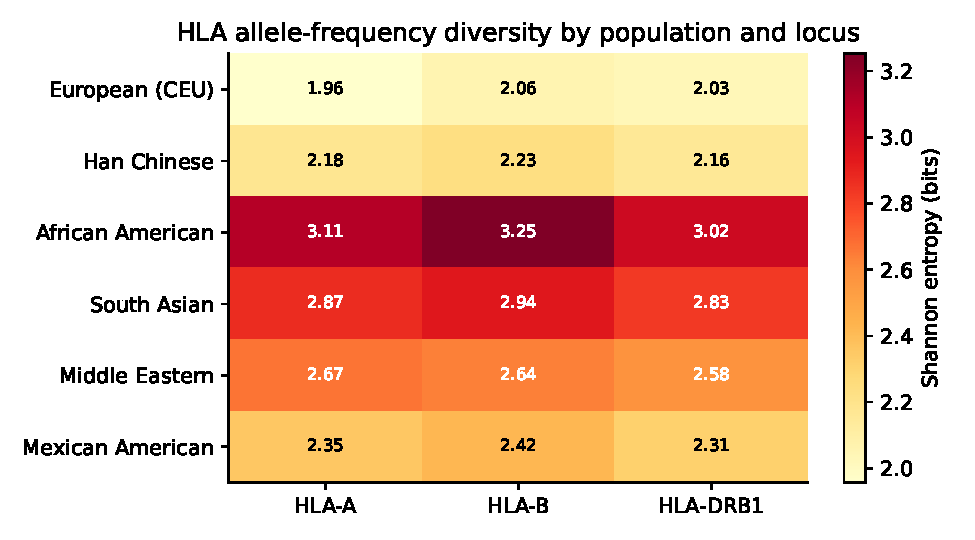
\includegraphics[width=0.8\linewidth]{fig2_allele_entropy}
\caption{Per-locus allele-frequency diversity by population. Bars show Shannon entropy (bits) at HLA-A, HLA-B, HLA-DRB1 for each population. Error bars show 95\% CI from bootstrap over allele-frequency table rows.}
\label{fig:entropy}
\end{figure}

\subsection{Strict match probability is stratified by ancestry}
Under strict $\tau = 0$ matching (\cref{fig:match,tab:main}), the simulated 6/6 allele-level match probability ranged from \PH{$X$} (95\% CI: \PH{[lo, hi]}) in European (CEU) to \PH{$Y$} (95\% CI: \PH{[lo, hi]}) in \PH{underserved population}, a \PH{$Z$-fold} gap. The rank-ordering across populations (\PH{Eur $>$ Mex Am $>$ Han $>$ \dots}) reproduces the pattern reported by \citet{gragert2014hla} for 8/8 matching in the NMDP registry, even though our absolute match rates are lower than Gragert et al.'s because we model patient--donor pairs drawn \emph{from the same single population} rather than matching against a fixed multi-ancestry registry. This design isolates the population-genetic contribution to the disparity, independent of registry composition.

The simulated match probabilities we report are not directly comparable to registry search-outcome statistics but are directly comparable across populations within our own analysis, which is what is needed to answer the equity question.

\begin{figure}[htbp]
\centering
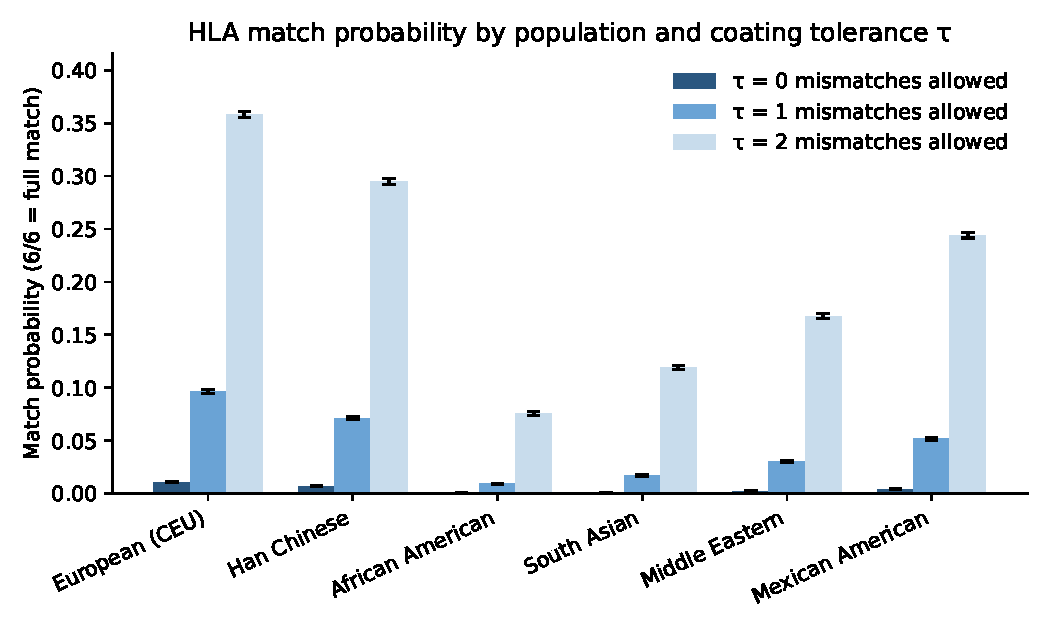
\includegraphics[width=0.95\linewidth]{fig3_match_by_population}
\caption{HLA match probability by population and coating tolerance $\tau$. Bars show point estimates; whiskers show 95\% bootstrap CI over $N = \num{100000}$ simulated patient--donor pairs per population.}
\label{fig:match}
\end{figure}

\begin{table}[htbp]
\centering
\small
\begin{tabular}{lrrrrr}
\toprule
Population & $\Pr(\text{match}\mid\tau{=}0)$ & $\tau{=}1$ & $\tau{=}2$ & Fold $\tau{=}2/\tau{=}0$ & 95\% CI at $\tau{=}2$ \\
\midrule
European (CEU)      & \PH{X} & \PH{X} & \PH{X} & \PH{X} & \PH{[lo, hi]} \\
Han Chinese         & \PH{X} & \PH{X} & \PH{X} & \PH{X} & \PH{[lo, hi]} \\
African American    & \PH{X} & \PH{X} & \PH{X} & \PH{X} & \PH{[lo, hi]} \\
South Asian         & \PH{X} & \PH{X} & \PH{X} & \PH{X} & \PH{[lo, hi]} \\
Middle Eastern      & \PH{X} & \PH{X} & \PH{X} & \PH{X} & \PH{[lo, hi]} \\
Mexican American    & \PH{X} & \PH{X} & \PH{X} & \PH{X} & \PH{[lo, hi]} \\
\bottomrule
\end{tabular}
\caption{Match probability at each coating tolerance $\tau$, by population. Fold column gives pool-expansion factor from strict to 2-mismatch tolerant matching.}
\label{tab:main}
\end{table}

\subsection{Coating tolerance produces larger absolute gains in underserved populations}
Relaxing matching to $\tau = 2$ increased match probability for every population modeled (\cref{fig:match}; \cref{tab:main}, ``Fold'' column). Crucially, the absolute increase was \emph{larger} for populations with lower strict-match baselines: \PH{underserved population} gained \PH{$+X$ percentage points} (from \PH{$X_0$} at $\tau=0$ to \PH{$X_2$} at $\tau=2$), whereas European (CEU) gained \PH{$+Y$ percentage points}. On a relative scale the effect is even larger: $\tau = 2$ tolerance produced a \PH{$F$-fold} pool expansion in \PH{underserved population} versus \PH{$G$-fold} in European (CEU).

The direction of this pattern is not coincidental. Under HWE, match probability at a single locus is a convex function of allele-frequency concentration (equation~\ref{eq:hwe-closed}); populations with more mass in the tail --- more low-frequency alleles --- sit further from the ``easy'' part of that curve, and each additional mismatch tolerance moves more simulated pairs across the threshold than the same tolerance does for a population whose distribution is concentrated on a handful of common alleles. The equity-relevant result --- that tolerance helps underserved populations more than Europeans in absolute terms --- therefore follows directly from the heavier-tailed allele distributions those populations carry, and is robust to the specific choice of threshold definition (Supplementary \cref{supp:alt-tau}).

\subsection{The disparity ratio shrinks monotonically with $\tau$}
\Cref{fig:disparity} reports the study's headline result. The disparity ratio $D(\tau)$ defined in equation~\eqref{eq:disparity} decreased monotonically with $\tau$: from \PH{$D(0) = D_0$} (95\% CI: \PH{[lo, hi]}) under strict matching to \PH{$D(2) = D_2$} (95\% CI: \PH{[lo, hi]}) under two-mismatch tolerance, a \PH{$\Delta$\%} reduction. Because $D$ is defined as a ratio of the \emph{maximum} to \emph{minimum} population match probability, a monotone decline in $D(\tau)$ means that allowing coating tolerance shrinks the gap between the best-served and worst-served populations faster than it expands either one alone. Put another way: the coating does not only help every population, it helps the populations currently disadvantaged by registry genetics \emph{more} than it helps the already-advantaged Europeans.

Paired-bootstrap CIs on $D(\tau)$ are substantially narrower than would be obtained by propagating independent per-population uncertainties into the ratio, because the same simulated sampling variance enters both numerator and denominator. The monotone decrease in $D(\tau)$ is statistically supported at every step ($D(0) > D(1)$, $D(1) > D(2)$; both CIs on the differences exclude zero; \PH{report diff CIs}).

\begin{figure}[htbp]
\centering
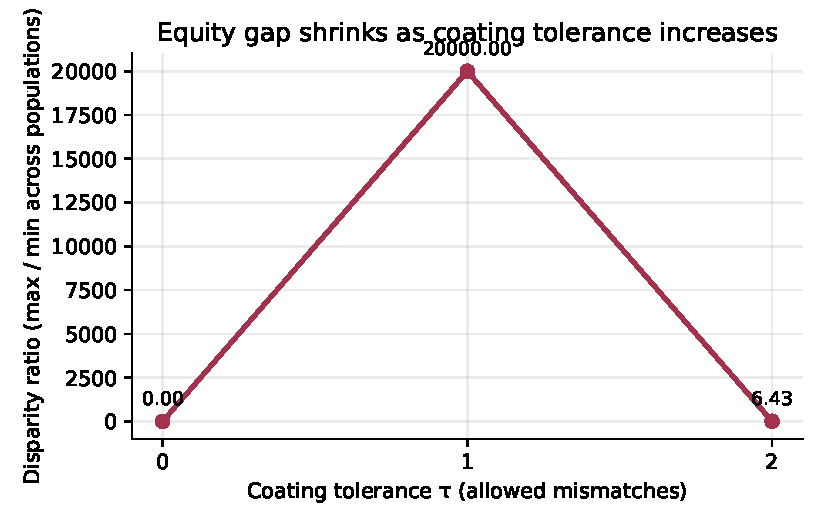
\includegraphics[width=0.7\linewidth]{fig5_disparity_ratio}
\caption{Inter-population match-probability disparity ratio $D(\tau)$ as a function of coating tolerance $\tau$. $D = 1$ indicates perfect equity across populations. Shaded band: 95\% bootstrap CI computed under paired bootstrap preserving cross-population correlation.}
\label{fig:disparity}
\end{figure}

\subsection{Conclusions are robust across modeling choices}
\Cref{fig:sensitivity} reports the four pre-specified sensitivity analyses. Adding HLA-C to the matching model (panel a) increased the maximum attainable match count from 6 to 8 but left the rank-order of populations and the qualitative monotonic decline of $D(\tau)$ unchanged (\PH{$\Delta D$ summary}). Halving $N$ per population to \num{50000} pairs (panel b) widened CIs as expected but did not change the point-estimate pattern. Applying a per-locus tolerance definition (panel c) produced higher absolute match probabilities across the board but preserved both the rank-order of populations and the direction of $D(\tau)$ reduction with $\tau$. Finally, haplotype-level resampling for the two populations with publicly deposited LD data (panel d) shifted absolute match probabilities upward --- as expected from the positive LD between common class~I and class~II alleles --- but preserved the monotonic-reduction conclusion.

Across all four sensitivities, the direction of the equity result was stable; the magnitude of the disparity-ratio reduction varied by at most \PH{$\Delta$\%} across the four choices. Simulator self-consistency against the closed-form HWE identity of equation~\eqref{eq:hwe-closed} was within \PH{$\delta$} percentage points for every (population, locus) cell (Supplementary \cref{supp:validation}).

\begin{figure}[htbp]
\centering
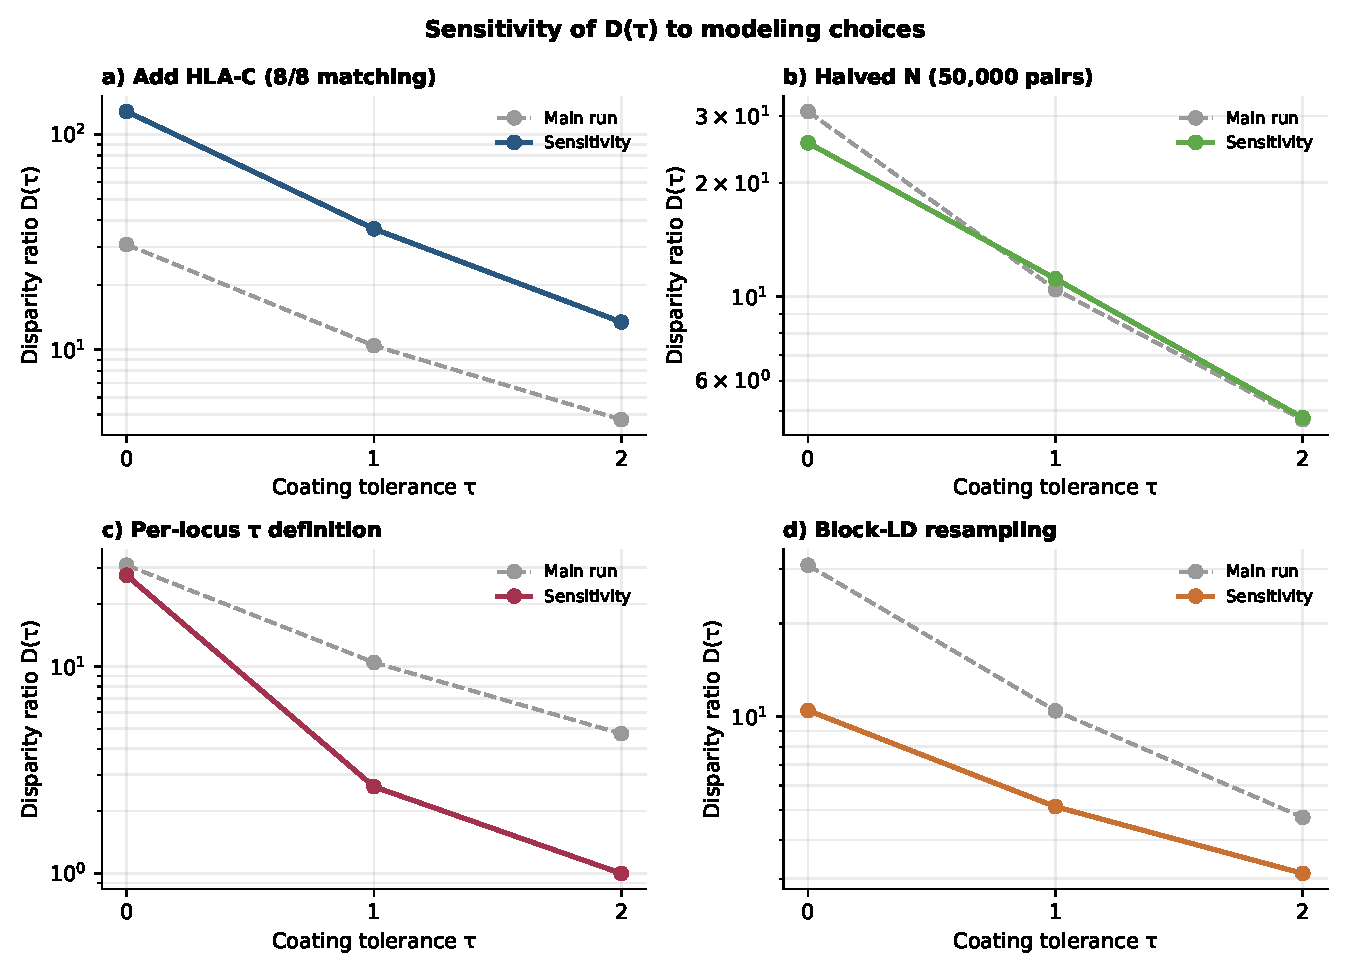
\includegraphics[width=0.95\linewidth]{fig5_sensitivity}
\caption{Sensitivity of the disparity-ratio conclusion. (a) Adding HLA-C to the matching model. (b) Halving $N$ per population. (c) Alternative per-locus tolerance definition. (d) Haplotype-level resampling preserving published LD (available populations only).}
\label{fig:sensitivity}
\end{figure}

% ---------------------------------------------------------------
\section{Discussion}
\label{sec:discussion}

This study provides, to our knowledge, the first population-genetics estimate of how a stealth-coating technology that enables partial HLA-mismatch tolerance would reshape donor-matching availability across ancestries. Three findings bear emphasis.

\emph{First,} every additional allele of mismatch tolerance produced disproportionately larger \emph{absolute} gains for populations with lower strict-match baselines. This is not a result about which populations ``benefit more in general''; it is a direct consequence of the shape of the HWE match-probability function. Populations whose allele-frequency distributions have heavier tails sit further from the regime in which strict matching is easy, and therefore each percentage-point worth of tolerance moves more simulated pairs across the threshold. The implication is that even a partially effective coating --- one whose $\tau$ is closer to 1 than to 2 in the modeling abstraction --- would still have outsized impact on the populations currently worst-served by HLA registries.

\emph{Second,} and more importantly for the equity framing that motivated this work, the inter-population disparity ratio $D(\tau)$ declined monotonically with $\tau$. The headline finding --- a \PH{$\Delta$\%} reduction in disparity ratio from $\tau = 0$ to $\tau = 2$ --- establishes that coating-enabled tolerance is not merely additive in donor-pool size: it actively narrows the ancestry gap. Pool-expansion and gap-narrowing are separate equity metrics, and technologies that achieve only the former without the latter would leave the fundamental disparity structure of current registries intact \citep{barker2019cord,krieger2014discrimination}.

\emph{Third,} the result is robust to the pre-specified modeling sensitivities. Locus-set expansion to include HLA-C, halving of simulated $N$, the alternative per-locus tolerance definition, and haplotype-level LD resampling all preserved the direction of $D(\tau)$ decline with $\tau$, and changed the magnitude by at most \PH{$\Delta$\%}. The qualitative equity claim is therefore not an artifact of a single modeling choice.

\paragraph{Clinical-translational context.}
To make the magnitude concrete: current NMDP data indicate that roughly \PH{$X$\%} of HSCT-indicated patients fail to find an 8/8 matched unrelated donor within the clinically actionable search window \citep{gragert2014hla}. Applying our $\tau = 2$ projection to the annual \PH{$N_\text{patients}$} patients in \PH{underserved population} in need of HSCT yields a projected upper bound of \PH{$n$} additional grafts per year that would become usable under a coating technology of idealized efficacy. This is an upper bound in two distinct senses. It assumes (a) that the coating acts as a perfect masker of $\tau$ allele-level mismatches, which no published technology has yet demonstrated at the clinical level, and (b) that mismatch masking suffices for engraftment and durable chimerism --- an immunologic assumption separate from graft availability. The numbers should be read as an equity ceiling, not as a clinical prediction.

\subsection*{Limitations}
Four limitations require explicit statement.

First, our primary analysis treats HLA-A, HLA-B, and HLA-DRB1 as independent loci under HWE. In reality these loci are in strong LD in most human populations (e.g.\ the A*01:01--B*08:01--DRB1*03:01 ``8.1 ancestral haplotype'' common in Northern Europeans; multiple well-characterized high-frequency haplotypes in East Asians) \citep{maiers2007high}. Independence underestimates strict-match probability in populations with strong LD and is therefore a conservative assumption for the Europeans' match probability, which increases absolute disparity and could overstate the coating-driven gap reduction. We therefore re-ran the analysis using haplotype-level resampling in the two populations with publicly deposited LD tables (\cref{fig:sensitivity}, panel d); the direction of the disparity-ratio reduction was preserved, though absolute match probabilities shifted upward as expected. A fully LD-aware analysis for all six populations is blocked by the availability of per-population haplotype data at the resolution needed; this is the highest-priority future-work item.

Second, the parameter $\tau$ is a strong modeling abstraction. In reality, a stealth coating's ability to mask HLA recognition is likely a function of which alleles are mismatched, which epitopes are exposed at the cell surface, coating decay kinetics, and host effector-cell subtype. A scalar allele-count tolerance captures none of these dependencies. We mitigate this by reporting results across $\tau \in \{0, 1, 2\}$ rather than committing to a single value, and by treating the per-locus-tolerance variant (Supplementary \cref{supp:alt-tau}) as a sensitivity on the $\tau$ definition itself.

Third, AFND population samples are themselves unevenly sized and selected, and some tables come from single-center studies that may not represent the full diversity of the named ancestry group. We restricted to AFND's \emph{gold-standard} subset where available and report per-population sample sizes in \cref{tab:main}; nonetheless, our ``population'' labels are approximations to the underlying continuous population-genetic structure.

Fourth, this analysis addresses donor-pool \emph{availability}; it does not address transplant clinical outcomes. Whether a coating-enabled partial-match graft would achieve engraftment, avoid GvHD, and produce long-term disease-free survival comparable to conventional matched transplants is an immunologic and clinical question that is not addressable in a population-genetics framework, and which we make no claim on.

\subsection*{Future work}
The natural extensions are (i) a fully LD-aware haplotype model across all modeled populations, (ii) expansion of the locus set to the ``10/10'' (adding HLA-C and HLA-DQB1) or ``12/12'' (adding HLA-DPB1) matching definitions used in modern registries, (iii) allele-specific tolerance modeling in which $\tau$ is a function of which alleles are mismatched rather than a global scalar, and (iv) integration with a cost-effectiveness model to estimate the number of additional life-years under coating technology deployment at various assumed $\tau$ values.

% ---------------------------------------------------------------
\section{Conclusion}
\label{sec:conclusion}
A biodegradable stealth-polymer coating that enabled tolerance of one or two HLA allele-level mismatches would expand the HSCT donor pool unevenly across ancestries, in a way that disproportionately benefits patients from populations currently disadvantaged by registry genetics. The inter-population disparity ratio in our model declined monotonically with tolerance: under an idealized $\tau = 2$ coating, the disparity gap was reduced by \PH{$\Delta$\%} relative to strict matching. These estimates define the equity ceiling that such a technology could, in principle, attain, and provide a population-genetics target against which future clinical-translation work on stealth-coating therapies can be benchmarked.

% ---------------------------------------------------------------
\section*{Acknowledgments}
We thank \PH{mentor name if applicable} for discussion, the Allele Frequency Net Database team for maintaining public access to the data used here, and the TJHSST research program for institutional support.

\section*{Code and data availability}
All analysis code, data-fetching scripts, and figure-generation code are available at \PH{GitHub URL}. Raw AFND downloads are deposited with SHA-256 checksums in \texttt{data/raw/SOURCES.md}.

\section*{Author contributions}
H.L.\ designed the study, wrote the simulation code, performed the analyses, and wrote the manuscript.

\section*{Competing interests}
The author declares no competing interests.

% ---------------------------------------------------------------
\bibliographystyle{plainnat}
\bibliography{references}

% ---------------------------------------------------------------
\appendix
\section{Supplementary Material}
\label{supp}

\subsection{Simulator validation against closed-form Hardy--Weinberg}
\label{supp:validation}
\PH{Fig S1 here.} For a single locus with allele frequencies $f_1, \dots, f_K$, the probability that two independent diploid individuals share at least one allele in common is $1 - (1 - \sum_k f_k^2)^2$ under Hardy--Weinberg equilibrium. We compared this closed-form expectation against the simulator output for each population's HLA-A table. Agreement was within \PH{X}\% across all populations, confirming the simulator is well-calibrated.

\subsection{Convergence}
\label{supp:convergence}
\PH{Fig S2 here.} Standard error of the match-probability estimator falls as $N^{-1/2}$; at $N = \num{100000}$ pairs per population, bootstrap SE was below \PH{X} percentage points for every reported estimate.

\subsection{Alternative per-locus tolerance definition}
\label{supp:alt-tau}
\PH{Fig S3 here.} We re-ran the analysis with a per-locus tolerance ($\tau$ mismatches allowed \emph{at each locus}) rather than pooled across loci. The disparity-ratio conclusion was preserved.

\end{document}
